% \chapter{The first appendix}

% Text for the first appendix goes here.

% \section{Appendix section}

\chapter{\ifenglish Manual For Installation\else คู่มือการติดตั้ง\fi}

\section{Next.js 14 (Frontend)}
\begin{figure}[H]
    \centering
    
\includegraphics[width=100mm, keepaspectratio ]{pictures/nextjs.png}
\end{figure}
โครงสร้างของโปรเจกต์นี้ประกอบด้วยหลายไฟล์และโฟลเดอร์ที่สำคัญสำหรับการพัฒนาและการตั้งค่าโปรเจกต์ โดยมีรายละเอียดดังนี้:

\subsection{Main Files and Folders}
\begin{itemize}
    \item \textbf{.dockerignore}: ไฟล์ที่ระบุไฟล์หรือโฟลเดอร์ที่ไม่ต้องการให้ Docker คัดลอกไปยัง image
    \item \textbf{.env, .env.local, .env.prod}: ไฟล์ที่ใช้เก็บค่าตัวแปรสภาพแวดล้อม (environment variables) สำหรับการตั้งค่าโปรเจกต์ในสภาพแวดล้อมต่างๆ
    \item \textbf{.eslintrc.json}: ไฟล์การตั้งค่า ESLint สำหรับการตรวจสอบและจัดรูปแบบโค้ด
    \item \textbf{.gitignore}: ไฟล์ที่ระบุไฟล์หรือโฟลเดอร์ที่ไม่ต้องการให้ Git ติดตาม
    \item \textbf{docker-compose.yml}: ไฟล์การตั้งค่า Docker Compose สำหรับการจัดการ container หลายๆ ตัว
    \item \textbf{Dockerfile}: ไฟล์การตั้งค่า Docker สำหรับการสร้าง Docker image
    \item \textbf{next-env.d.ts}: ไฟล์การตั้งค่า TypeScript สำหรับโปรเจกต์ Next.js
    \item \textbf{next.config.mjs}: ไฟล์การตั้งค่า Next.js
    \item \textbf{package.json}: ไฟล์ที่เก็บข้อมูลเกี่ยวกับโปรเจกต์ Node.js รวมถึง dependencies และสคริปต์ต่างๆ
    \item \textbf{postcss.config.mjs}: ไฟล์การตั้งค่า PostCSS
    \item \textbf{README.md}: ไฟล์เอกสารสำหรับโปรเจกต์
    \item \textbf{tailwind.config.ts}: ไฟล์การตั้งค่า Tailwind CSS
    \item \textbf{tsconfig.json}: ไฟล์การตั้งค่า TypeScript
\end{itemize}

\subsection{Subfolders}
\begin{itemize}
    \item \textbf{workflows}: โฟลเดอร์ที่เก็บไฟล์การตั้งค่า GitHub Actions สำหรับการทำงานอัตโนมัติ
    \item \textbf{.next}: โฟลเดอร์ที่เก็บไฟล์ที่ถูกสร้างขึ้นโดย Next.js หลังจากการ build
    \item \textbf{.vs}: โฟลเดอร์ที่เก็บการตั้งค่าของ Visual Studio Code
    \item \textbf{app}: โฟลเดอร์ที่เก็บไฟล์และโฟลเดอร์ที่เกี่ยวข้องกับการทำงานของแอปพลิเคชัน
    \item \textbf{components}: โฟลเดอร์ที่เก็บคอมโพเนนต์ React ที่ใช้ในโปรเจกต์
    \item \textbf{config}: โฟลเดอร์ที่เก็บไฟล์การตั้งค่าต่างๆ
    \item \textbf{context}: โฟลเดอร์ที่เก็บไฟล์ context ของ React
    \item \textbf{dtos}: โฟลเดอร์ที่เก็บไฟล์ Data Transfer Objects (DTOs)
    \item \textbf{hooks}: โฟลเดอร์ที่เก็บ custom hooks ของ React
    \item \textbf{models}: โฟลเดอร์ที่เก็บไฟล์โมเดลต่างๆ
    \item \textbf{pages}: โฟลเดอร์ที่เก็บไฟล์เพจของ Next.js
    \item \textbf{public}: โฟลเดอร์ที่เก็บไฟล์สาธารณะ เช่น รูปภาพ
    \item \textbf{types}: โฟลเดอร์ที่เก็บไฟล์ประเภท (types) ของ TypeScript
    \item \textbf{utils}: โฟลเดอร์ที่เก็บไฟล์ utility functions
\end{itemize}

\section{Installation Guide}
\subsection{Clone the Project from GitHub}
\begin{verbatim}
git clone https://github.com/259492-ProjectBox/frontend-projectbox.git
cd <repository-directory>
\end{verbatim}

\subsection{Install Dependencies}
\begin{verbatim}
npm install
\end{verbatim}

\subsection{Set Up Environment Variables}
สร้างไฟล์ \texttt{.env.local} และกำหนดค่าตัวแปรสภาพแวดล้อมตามที่ต้องการ

\subsection{Run the Project in Development Mode}
\begin{verbatim}
npm run dev
\end{verbatim}

\subsection{Build Docker Image (Optional)}
\begin{verbatim}
docker build -t <image-name> .
\end{verbatim}

\section{Elysia (Auth\_service)}
\begin{figure}[H]
    \centering
    
\includegraphics[width=100mm, keepaspectratio ]{pictures/elysia.jpg}
\end{figure}

\subsection{Project Structure}
รายละเอียดของไฟล์และโฟลเดอร์หลัก:
\begin{itemize}
    \item \textbf{.env}: ไฟล์นี้ใช้สำหรับเก็บค่าตัวแปรสภาพแวดล้อม เช่น ข้อมูลการเชื่อมต่อฐานข้อมูล และคีย์ลับต่างๆ
    \item \textbf{Dockerfile}: ไฟล์นี้ใช้สำหรับสร้าง Docker image ของโปรเจกต์
    \item \textbf{docker-compose.yml และ docker-compose.prod.yml}: ไฟล์นี้ใช้สำหรับการตั้งค่า Docker Compose เพื่อรันบริการต่างๆ ที่จำเป็นสำหรับโปรเจกต์
    \item \textbf{drizzle/}: โฟลเดอร์นี้เก็บไฟล์ที่เกี่ยวข้องกับการจัดการฐานข้อมูล เช่น สคีมาและการย้ายข้อมูล
    \item \textbf{src/}: โฟลเดอร์นี้เก็บโค้ดหลักของโปรเจกต์ แบ่งออกเป็นหลายโฟลเดอร์ย่อย เช่น controllers, dtos, middleware, repositories, services
    \item \textbf{types/}: โฟลเดอร์นี้เก็บไฟล์ที่ประกาศประเภทข้อมูลต่างๆ
    \item \textbf{utils/}: โฟลเดอร์นี้เก็บไฟล์ที่มีฟังก์ชันช่วยเหลือต่างๆ
\end{itemize}

\subsection{Installation and Usage}
\begin{enumerate}
    \item \textbf{ติดตั้ง Bun:}
    \begin{verbatim}
    Bun Installation 
    https://bun.sh/docs/installation
    \end{verbatim}
    \item \textbf{ติดตั้ง Dependencies:}
    \begin{verbatim}
    bun install
    \end{verbatim}
    \item \textbf{ตั้งค่าฐานข้อมูล:}
    \begin{itemize}
        \item ตรวจสอบให้แน่ใจว่าไฟล์ .env มีค่าตัวแปรสภาพแวดล้อมที่ถูกต้องสำหรับการเชื่อมต่อฐานข้อมูล
        \item รันคำสั่งต่อไปนี้เพื่อสร้างและตั้งค่าฐานข้อมูล:
    \end{itemize}
    \item \textbf{รันโปรเจกต์ในโหมดพัฒนา:}
    \begin{verbatim}
    bun run dev
    \end{verbatim}
\end{enumerate}

\section{Golang Project (Project\_service)}
\begin{figure}[H]
    \centering
    
\includegraphics[width=100mm, keepaspectratio ]{pictures/golang.png}
\end{figure}
\subsection{Project Structure}
รายละเอียดของไฟล์และโฟลเดอร์หลัก:
\begin{itemize}
    \item \textbf{.env.example}: ไฟล์นี้ใช้สำหรับเป็นตัวอย่างไฟล์สำหรับไฟล์ .env ในการเก็บค่าตัวแปรสภาพแวดล้อม เช่น ข้อมูลการเชื่อมต่อฐานข้อมูล และคีย์ลับต่างๆ
    \item \textbf{Dockerfile}: ไฟล์นี้ใช้สำหรับสร้าง Docker image ของโปรเจกต์
    \item \textbf{docker-compose.yml และ docker-compose.prod.yml}: ไฟล์นี้ใช้สำหรับการตั้งค่า Docker Compose เพื่อรันบริการต่างๆ ที่จำเป็นสำหรับโปรเจกต์
    \item \textbf{configs/}: โฟลเดอร์นี้เก็บ config ของ โปรเจกต์
    \item \textbf{db/}: โฟลเดอร์นี้เก็บไฟล์ที่เกี่ยวข้องกับการจัดการฐานข้อมูล เช่น สคีมาและการย้ายข้อมูล การเชื่อมต่อฐานข้อมูลต่างๆ
    \item \textbf{docs/}: โฟลเดอร์นี้เก็บไฟล์ API Documentation ของโปรเจกต์
    \item \textbf{routers/}: โฟลเดอร์นี้เก็บไฟล์ router ของโปรเจกต์เพื่อ routing request จาก client
    \item \textbf{handlers/}: โฟลเดอร์นี้เก็บไฟล์ handler ของโปรเจกต์สำหรับรับส่ง request จาก client
    \item \textbf{models/}: โฟลเดอร์นี้เก็บไฟล์โมเดลต่างๆ
    \item \textbf{services/}: โฟลเดอร์นี้เก็บไฟล์ที่เกี่ยวข้องกับการจัดการ logic ของโปรเจกต์
    \item \textbf{repositories/}: โฟลเดอร์นี้เก็บไฟล์ที่เกี่ยวข้องกับการจัดการข้อมูลในฐานข้อมูล
    \item \textbf{queues/}: โฟลเดอร์นี้เก็บไฟล์ที่เกี่ยวข้องกับการจัดการ queue ของโปรเจกต์
    \item \textbf{utils/}: โฟลเดอร์นี้เก็บไฟล์ที่มีฟังก์ชันช่วยเหลือต่างๆ
\end{itemize}

\subsection{Installation and Usage}
\begin{enumerate}
    \item \textbf{ติดตั้ง Golang:}
    \begin{verbatim}
    Golang Installation 
    https://go.dev/doc/install
    \end{verbatim}
    \item \textbf{ติดตั้ง Dependencies:}
    \begin{verbatim}
    go mod tidy
    \end{verbatim}
    \item \textbf{ติดตั้ง Dependencies เพิ่มเติม:}
    \begin{itemize}
        \item go install github.com/air-verse/air@latest
        \item go install github.com/swaggo/swag/cmd/swag@latest:
        \item scoop install poppler:
    \end{itemize}
    \item \textbf{ตั้งค่าฐานข้อมูล:}
    \begin{itemize}
        \item ตรวจสอบให้แน่ใจว่าไฟล์ .env มีค่าตัวแปรสภาพแวดล้อมที่ถูกต้องสำหรับการเชื่อมต่อฐานข้อมูล
        \item รันคำสั่งต่อไปนี้เพื่อสร้าง container ของฐานข้อมูล:
        \begin{verbatim}
        docker compose up -d
        \end{verbatim}
    \end{itemize}
    \item \textbf{รันโปรเจกต์:}
    \begin{verbatim}
    air
    \end{verbatim}
\end{enumerate}

\section{Java Project (Search\_service)}
\begin{figure}[H]
    \centering
    
\includegraphics[width=100mm, keepaspectratio ]{pictures/springboot.png}
\end{figure}
\subsection{Project Structure}
รายละเอียดของไฟล์และโฟลเดอร์หลัก:
\begin{itemize}
    \item \textbf{configs/}: โฟลเดอร์นี้เก็บ config ของ โปรเจกต์ เช่น Cors, RabbitMQ
    \item \textbf{consumers/}: โฟลเดอร์นี้เก็บไฟล์ที่เกี่ยวข้องกับการ consume message จาก Message Broker เช่น RabbitMQ
    \item \textbf{controllers/}: โฟลเดอร์นี้เก็บไฟล์ handler ของโปรเจกต์สำหรับรับส่ง request จาก client
    \item \textbf{db/}: โฟลเดอร์นี้เก็บไฟล์ที่เกี่ยวข้องกับการจัดการฐานข้อมูล เช่น การเชื่อมต่อฐานข้อมูลต่างๆ
    \item \textbf{models/}: โฟลเดอร์นี้เก็บไฟล์โมเดลต่างๆ
    \item \textbf{dtos/}: โฟลเดอร์นี้เก็บไฟล์ dto สำหรับการจัดการสร้าง object ของโปรเจกต์
    \item \textbf{services/}: โฟลเดอร์นี้เก็บไฟล์ที่เกี่ยวข้องกับการจัดการ logic ของโปรเจกต์
    \item \textbf{repositories/}: โฟลเดอร์นี้เก็บไฟล์ที่เกี่ยวข้องกับการจัดการข้อมูลในฐานข้อมูล
\end{itemize}

\subsection{Installation and Usage}
\begin{enumerate}
    \item \textbf{ติดตั้ง Java:}
    \begin{verbatim}
    Java Installation 
    https://www.java.com/en/download/help/windows_manual_download.html
    \end{verbatim}
    \item \textbf{ติดตั้ง Dependencies:}
    \begin{verbatim}
    mvn clean install
    \end{verbatim}
    \item \textbf{ตั้งค่าฐานข้อมูล:}
    \begin{itemize}
        \item ตรวจสอบให้แน่ใจว่าไฟล์ src/main/resources/application-dev.properties มีค่าตัวแปรสภาพแวดล้อมที่ถูกต้องสำหรับการเชื่อมต่อฐานข้อมูล
        \item รันคำสั่งต่อไปนี้เพื่อสร้าง container ของฐานข้อมูล:
        \begin{verbatim}
        docker compose up -d
        \end{verbatim}
    \end{itemize}
    \item \textbf{รันโปรเจกต์:}
    \begin{verbatim}
    mvn spring-boot:run
    \end{verbatim}
\end{enumerate}

\chapter{\ifenglish Manual\else คู่มือการใช้งานระบบ\fi}
% begin itemize with number
\begin{itemize}
    \item \textbf{\Large การใช้งานในส่วนของ User ทั่วไป}
\begin{enumerate}
    \item ทำการ Login เข้าสู่ระบบผ่าน CMU Account หรือ สามารถค้นหาโปรเจ็คได้โดยไม่ต้อง Login 
    % make it to call image
    \begin{figure}[H]
    \centering
    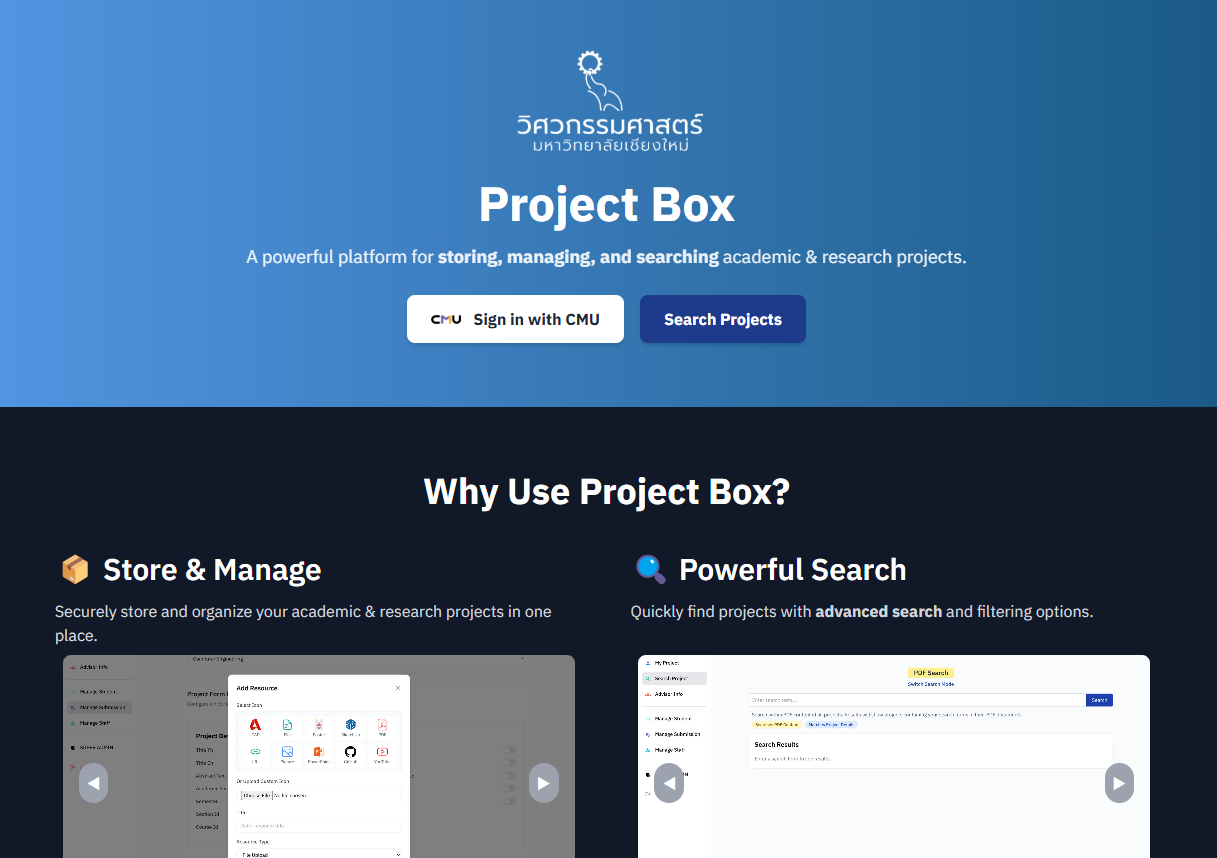
\includegraphics[width=130mm, keepaspectratio ]{pictures/project_box/loginpage.png}
    \end{figure}
    % space between image and text
    \vspace{1cm}
    \item เมื่อทำการ Login สำเร็จ จะเข้าสู่หน้า Dashboard ที่แสดงโปรเจ็คที่เคยสร้างไว้แล้ว หรือสามารถสร้างโปรเจ็คใหม่ได้เมื่อมีการลงทะเบียนเข้าใช้งาน
    \begin{figure}[H]
        \centering
        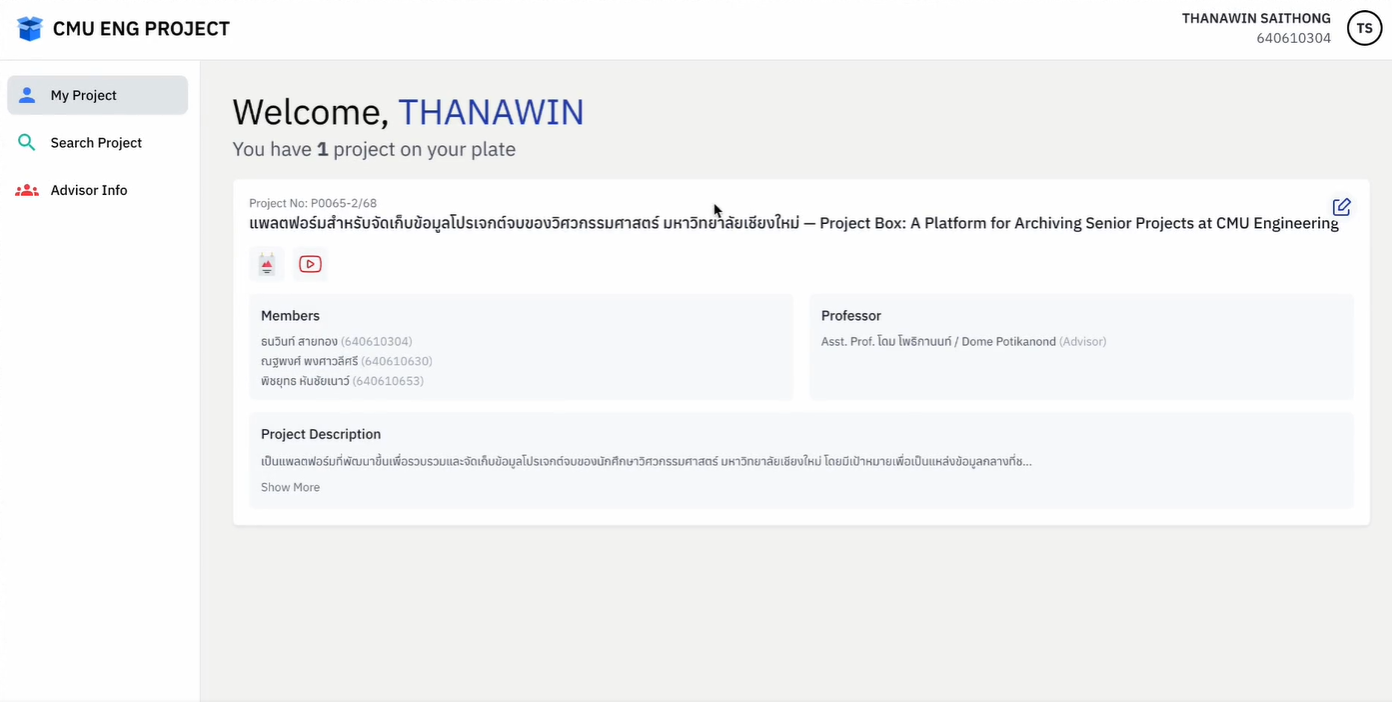
\includegraphics[width=130mm, keepaspectratio ]{pictures/project_box/dashboard.png
        }
    \end{figure}
    % new page after this 
    \newpage
    \item การค้นหาโปรเจ็ค สามารถค้นหาโปรเจ็คที่ต้องการได้จากช่องค้นหาโครงงาน 
    \begin{enumerate}
        \item Qucik Search ใช้การค้นหาโครงงานแบบง่าย
        \begin{figure}[H]
            \centering
            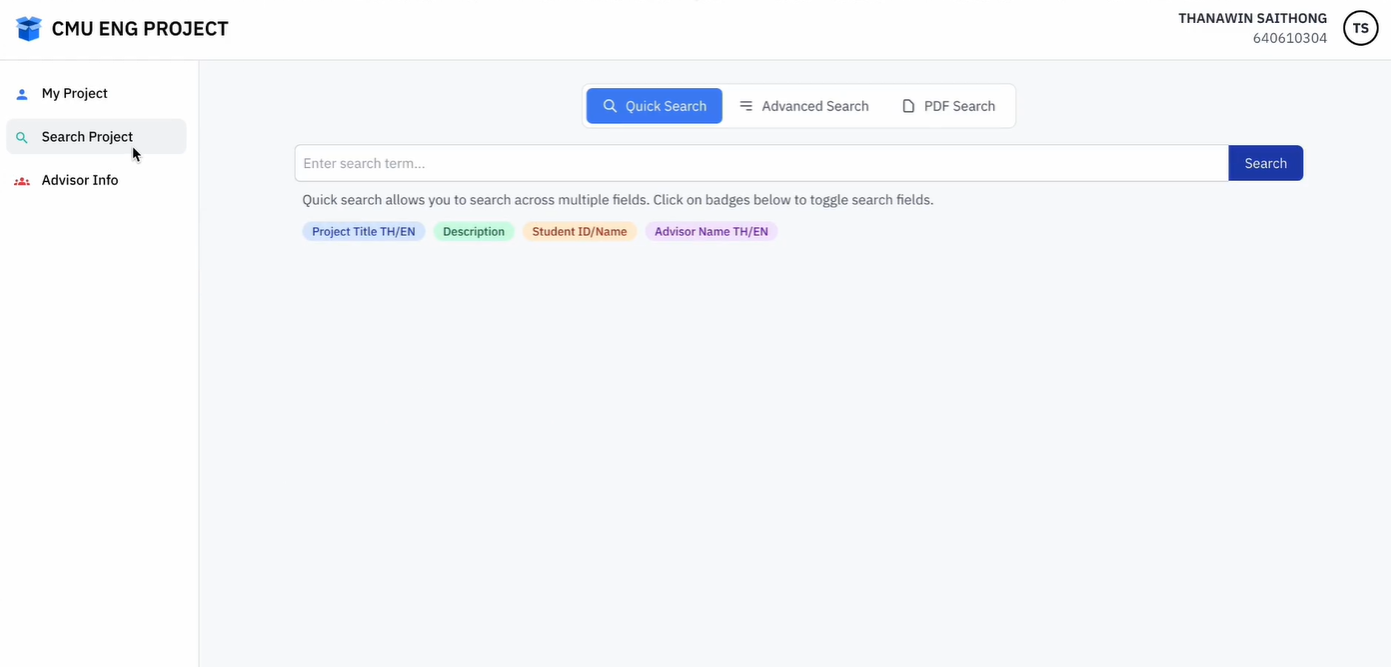
\includegraphics[width=130mm, keepaspectratio ]{pictures/project_box/quick_search.png}
        \end{figure}
        \item Advanced Search ใช้การค้นหาโครงงานแบบละเอียด
        \begin{figure}[H]
            \centering
            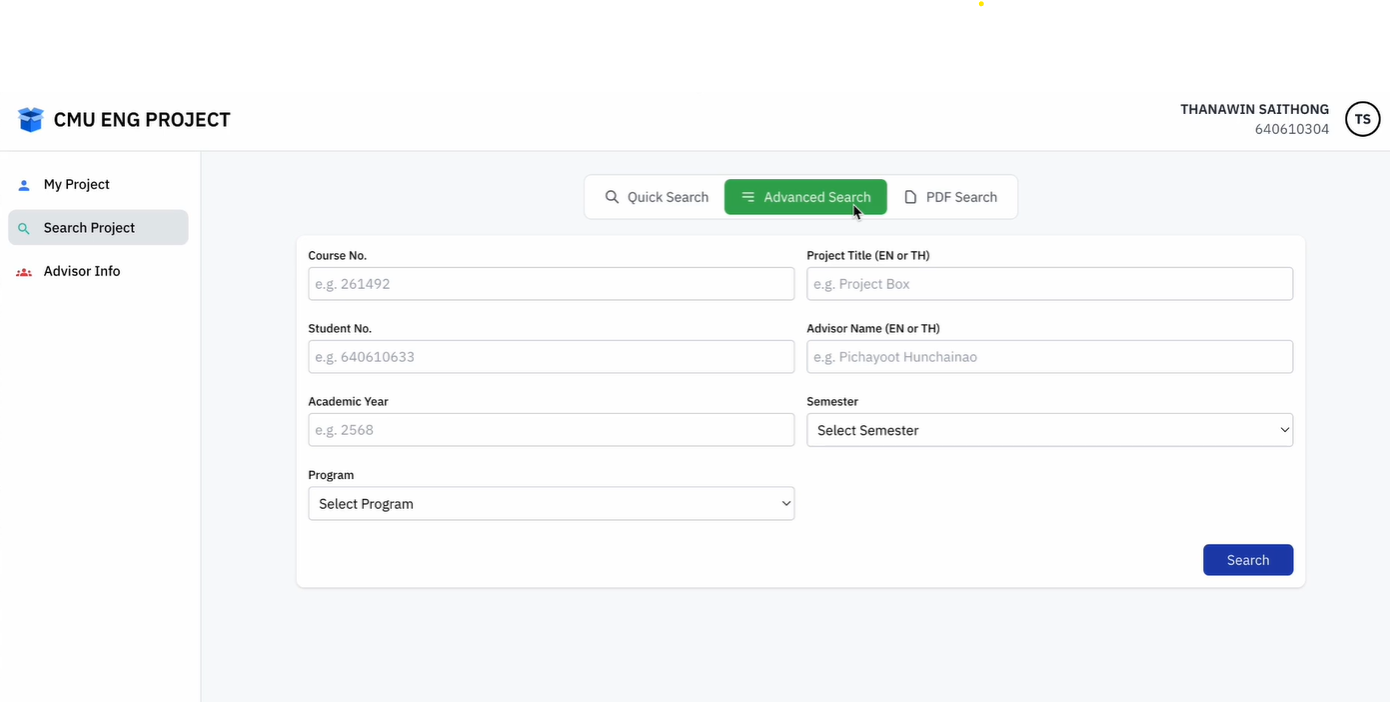
\includegraphics[width=130mm, keepaspectratio ]{pictures/project_box/advance_search.png}
        \end{figure} 
        \item PDF Search ใช้การค้นหาโครงงานจากไฟล์ PDF
        \begin{figure}[H]
            \centering
            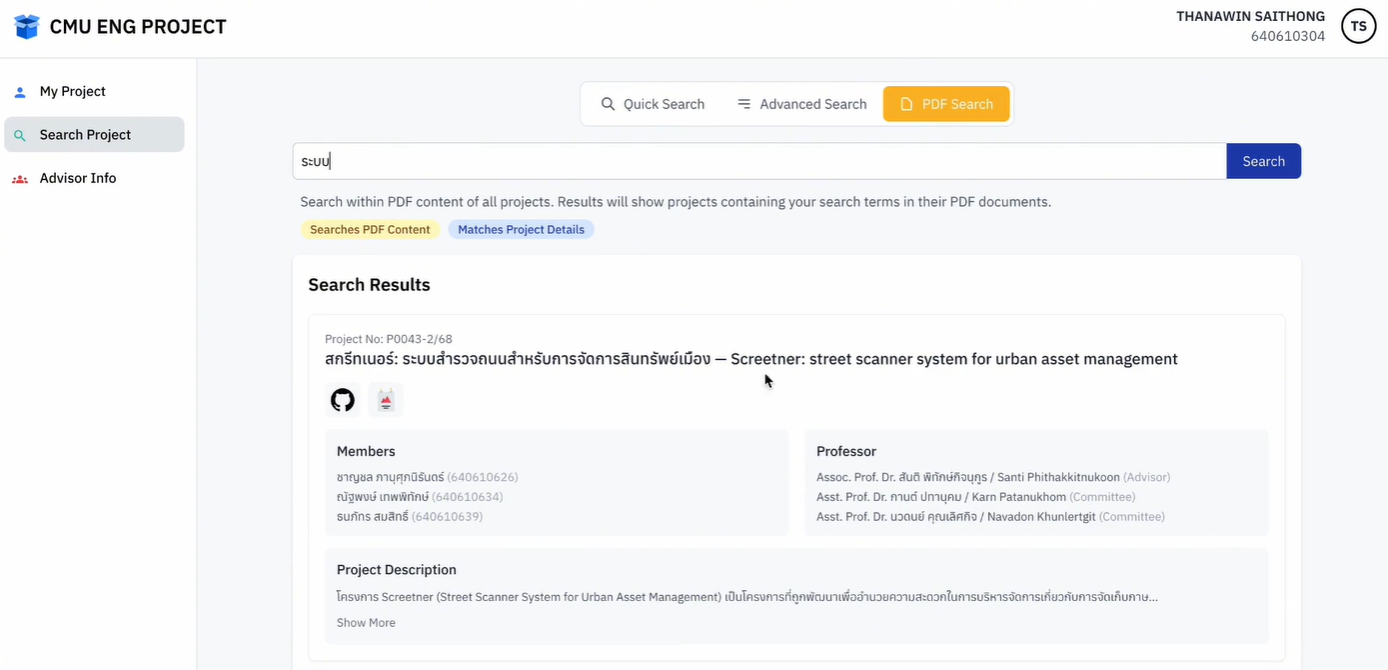
\includegraphics[width=130mm, keepaspectratio ]{pictures/project_box/pdf_search.png}
        \end{figure} 
        \item Keyword Search ใช้การค้นหาโครงงานจาก Keyword
        \begin{figure}[H]
            \centering
            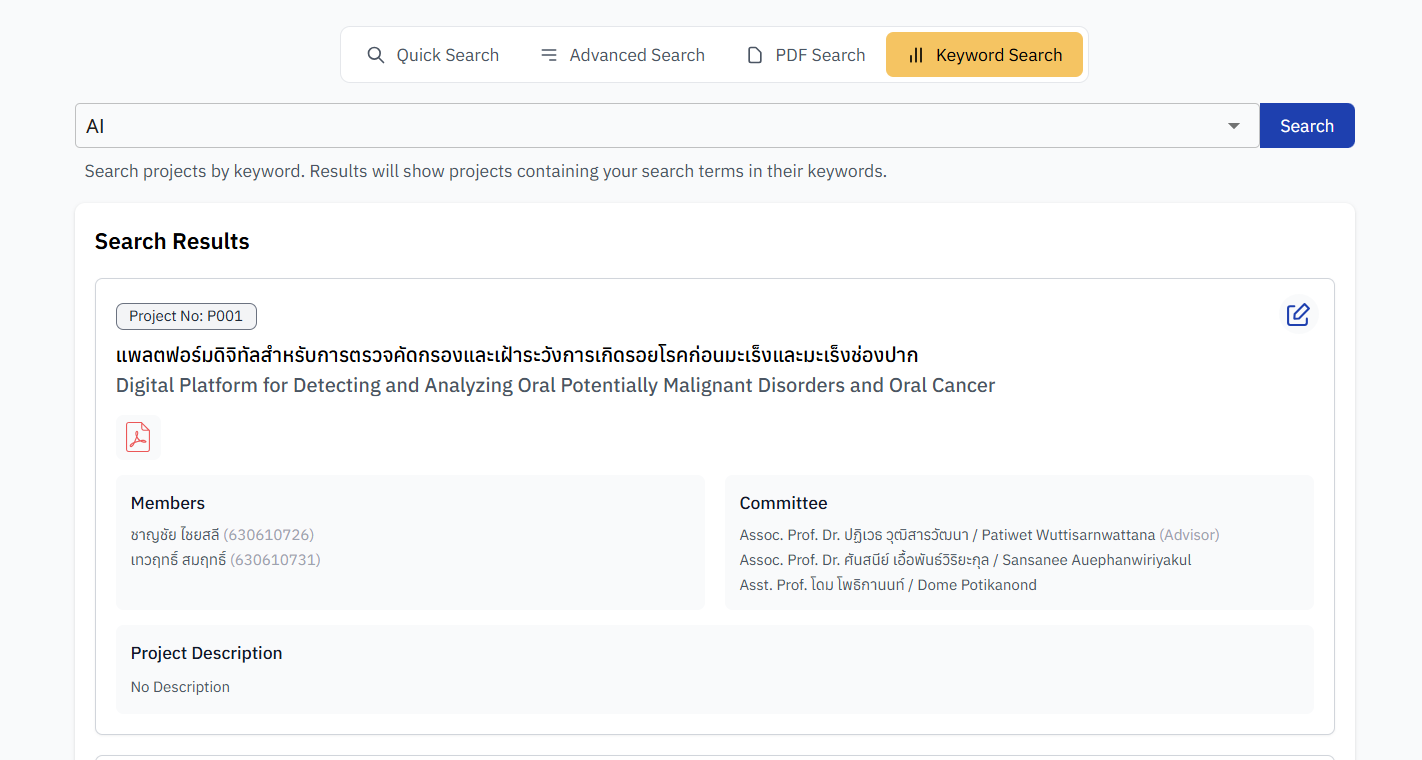
\includegraphics[width=130mm, keepaspectratio ]{pictures/project_box/keyword_search.png}
        \end{figure}
    \end{enumerate}
    \item ค้นหา Advisor Information สามารถค้นหาข้อมูลของอาจารย์ที่เกี่ยวข้องกับโครงงานได้
    \begin{enumerate}
        \item เลือกสาจารย์ที่ต้องการค้นหา
        \begin{figure}[H]
            \centering
            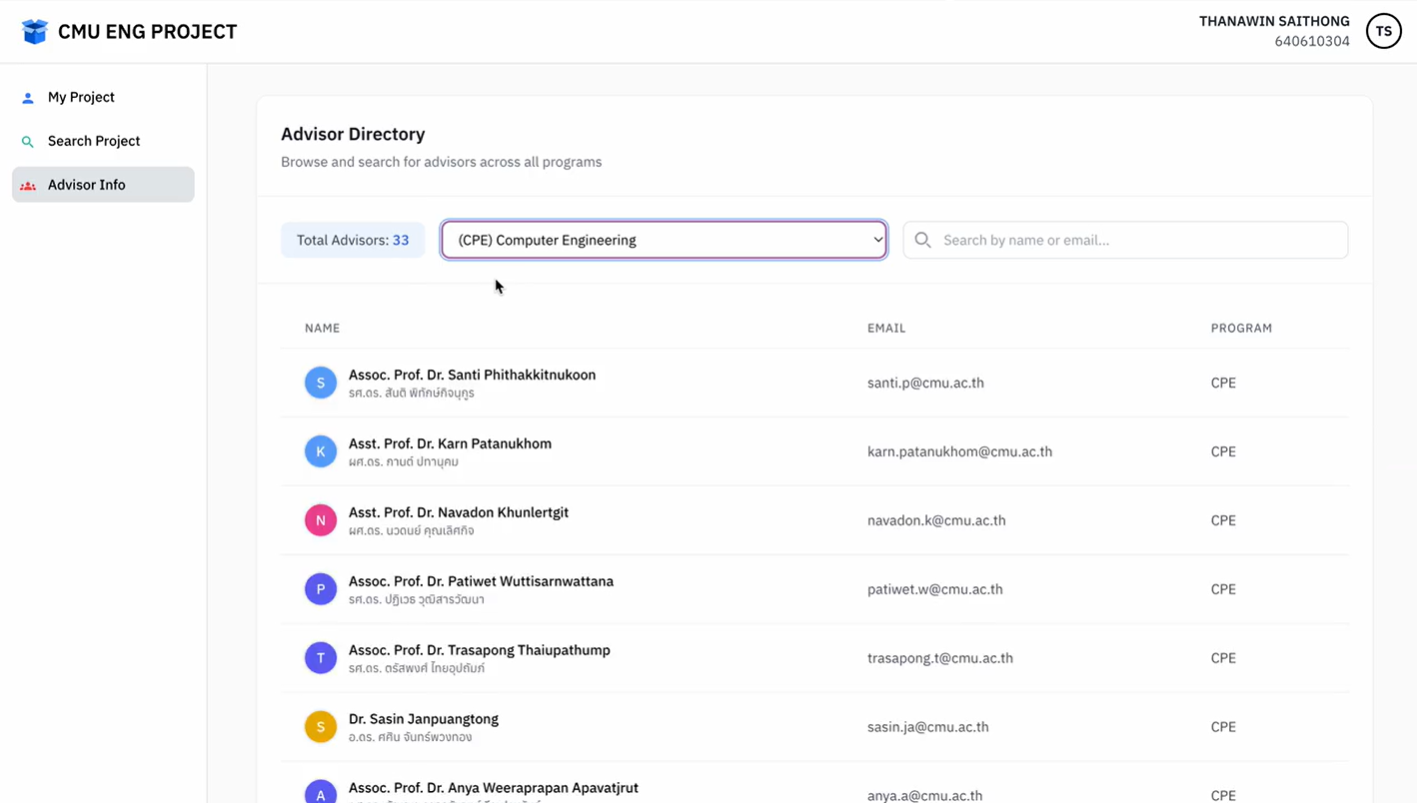
\includegraphics[width=130mm, keepaspectratio ]{pictures/project_box/advisor_info.png}
        \end{figure} 
        \item ดูข้อมูลของอาจารย์ว่าเลยเป็นที่ปรึกษาหรือกรรมการของโครงงานไหนบ้าง
        \begin{figure}[H]
            \centering
            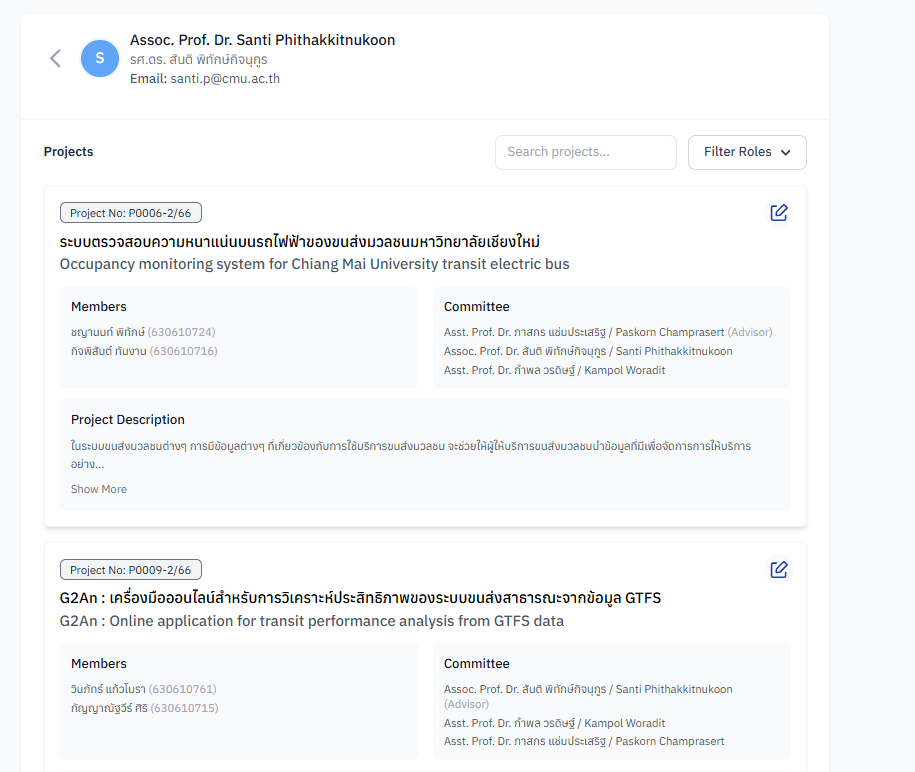
\includegraphics[width=130mm, keepaspectratio ]{pictures/project_box/advisor_project_involvement.png}
        \end{figure} 
    \end{enumerate}
    \item สร้างโครงงาน สามารถสร้างโครงงานใหม่ได้โดยการกดปุ่ม Create Project และกรอกข้อมูลต่างๆที่เกี่ยวข้องกับโครงงาน
    \begin{figure}[H]
        \centering
        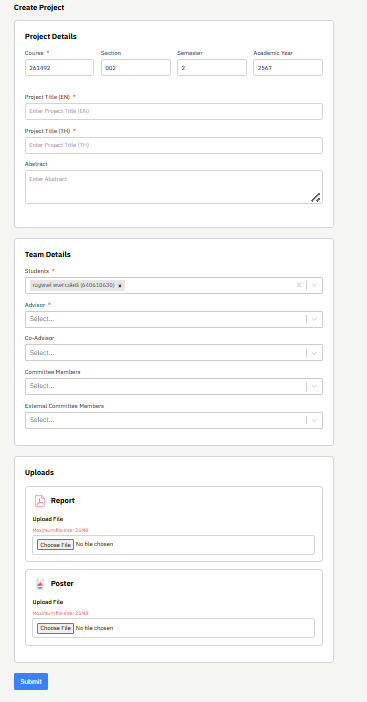
\includegraphics[width=130mm, keepaspectratio ]{pictures/project_box/create_project.png}
    \end{figure} 
\end{enumerate}
\newpage
\item \textbf{\Large การใช้งานในส่วนของเจ้าหน้าที่ปะจำสาขา Program Admin}
\begin{figure}[H]
    \centering
    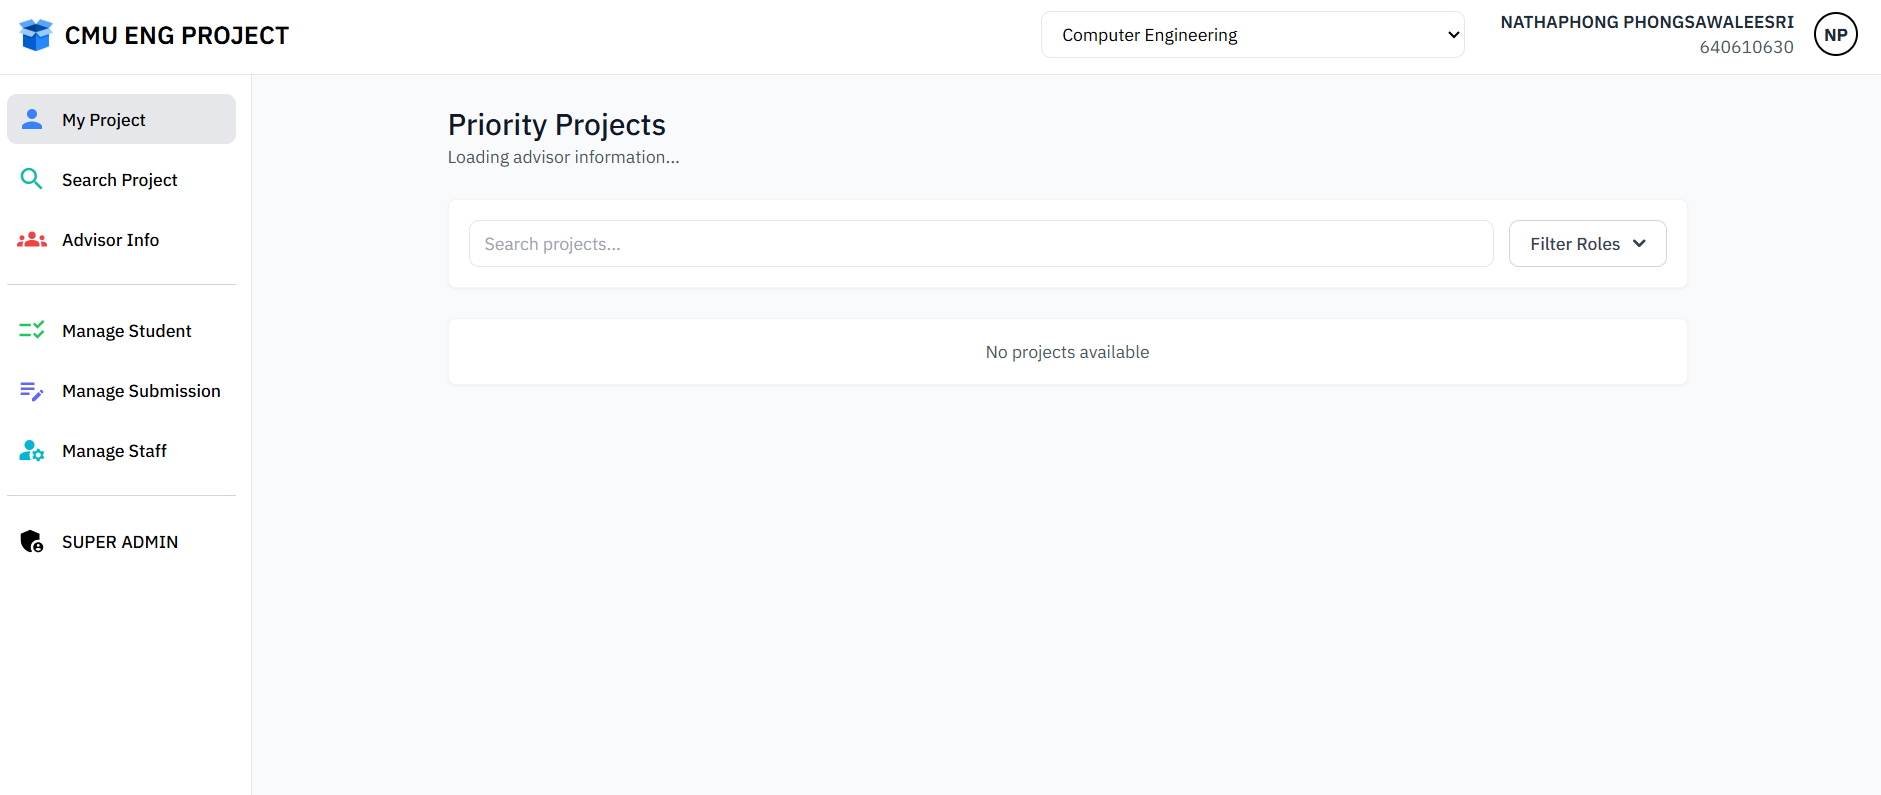
\includegraphics[width=130mm, keepaspectratio ]{pictures/project_box/program_admin_dashboard.png}
\end{figure}
\begin{enumerate}
    \item เลือก Program ที่ต้องการจัดการโครงงาน
    \begin{figure}[H]
        \centering
        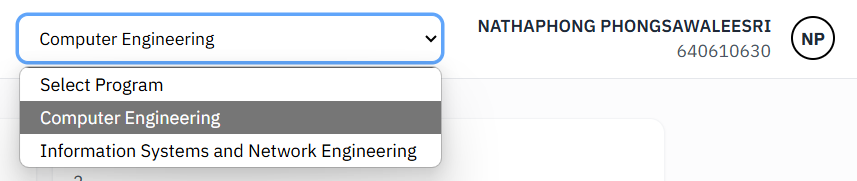
\includegraphics[width=130mm, keepaspectratio ]{pictures/project_box/select_program_before_manage.png}
    \end{figure}
    \item \textbf{จัดการนักศึกษา (Manage Student): } เจ้าหน้าที่สามารถจัดการข้อมูลนักศึกษาและสิทธิ์ในการสร้างโครงงานได้ โดยคลิกที่ปุ่ม "Manage Student" เพื่อเพิ่ม หรือตรวจสอบข้อมูลนักศึกษาว่ามีสิทธิ์ในการสร้างโครงงานในปีการศึกษาและภาคการศึกษานั้นๆ่
    \begin{enumerate}
        \item \textbf{เพิ่มข้อมูลนักศึกษา} เจ้าหน้าที่สามารถเพิ่มรายชื่อนักศึกษาเข้าสู่ระบบได้ โดยการนำเข้าข้อมูลจากไฟล์ Excel ที่ได้จากสำนักทะเบียน
        \begin{figure}[H]
            \centering
            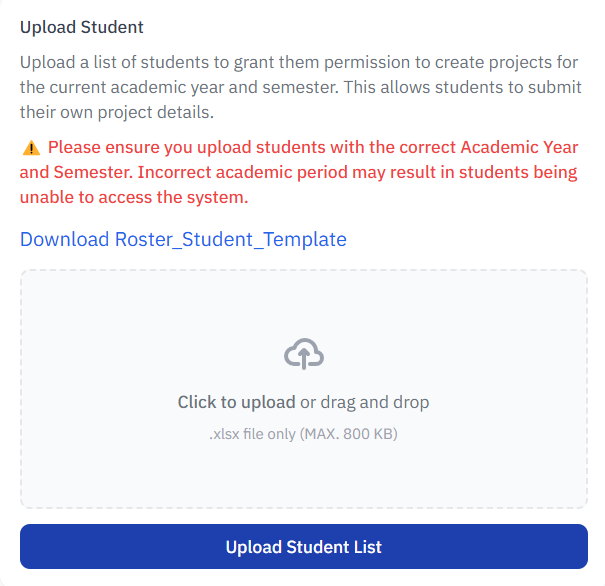
\includegraphics[width=100mm, keepaspectratio ]{pictures/project_box/add_new_student.png}
        \end{figure}
        \begin{figure}[H]
            \centering
            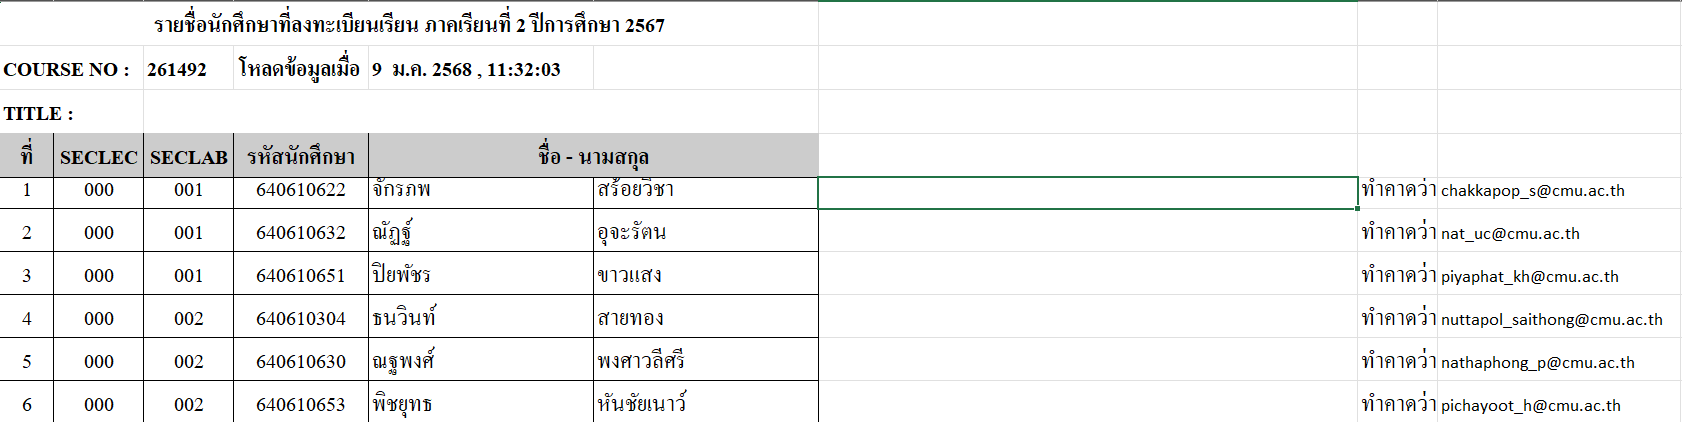
\includegraphics[width=100mm, keepaspectratio ]{pictures/project_box/student_template.png}
            \caption{ตัวอย่างไฟล์ Excel สำหรับนำเข้าข้อมูลนักศึกษา}
        \end{figure}
        \item \textbf{จัดการโครงงาน}: เจ้าหน้าที่สามารถดำเนินการดังนี้
        \begin{enumerate}
            \item \textbf{สร้างโครงงานเก่า}: เพิ่มข้อมูลโครงงานที่นักศึกษาเคยทำไว้แล้วในอดีต
            \item \textbf{มอบหมายโครงงาน}: เพิ่มโครงงานใหม่และกำหนดให้นักศึกษาดำเนินการ โดยนักศึกษาไม่จำเป็นต้องสร้างโครงงานเอง
        \end{enumerate}

        
        \begin{figure}[H]
            \centering
            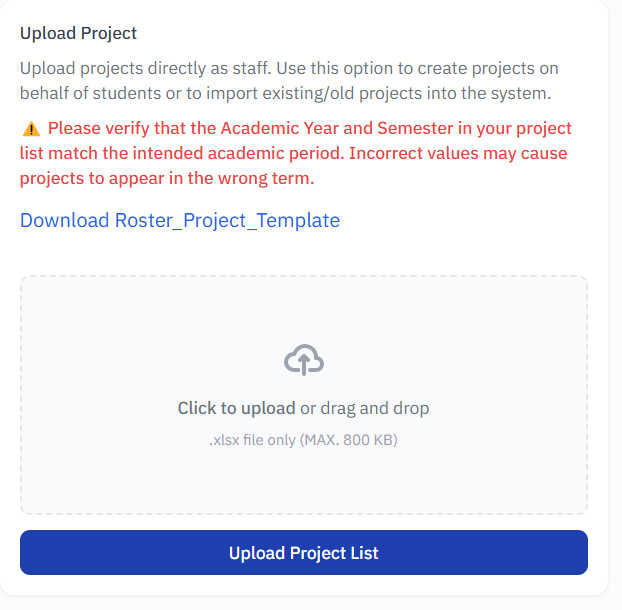
\includegraphics[width=100mm, keepaspectratio ]{pictures/project_box/upload_project_excel.png}
        \end{figure}
        \begin{figure}[H]
            \centering
            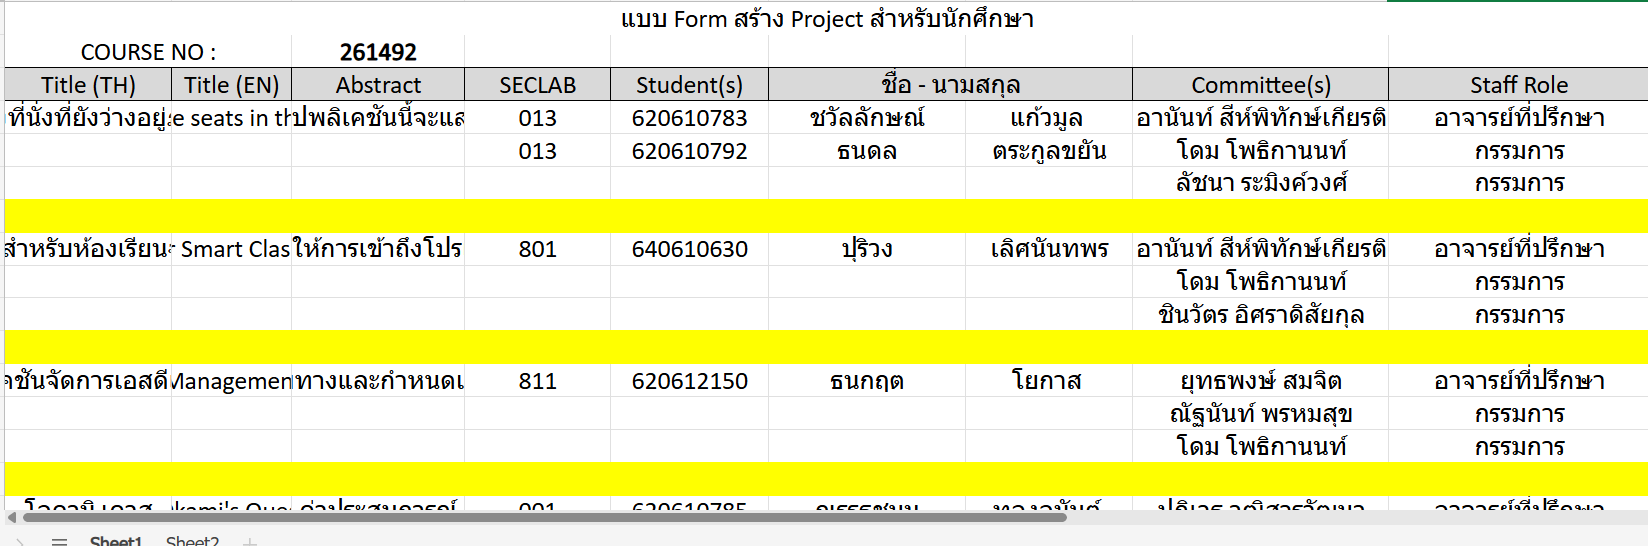
\includegraphics[width=100mm, keepaspectratio ]{pictures/project_box/create_project_template.png}
            \caption{ตัวอย่างไฟล์ Excel สำหรับนำเข้าข้อมูลโครงงาน}
        \end{figure}
    \end{enumerate}

    \newpage
    \item \textbf{จัดการรูปแบบการส่งโครงงาน (Manage Submission): } เจ้าหน้าที่สามารถกำหนดรูปแบบการส่งโครงงานให้กับนักศึกษาได้
    \begin{figure}[H]
        \centering
        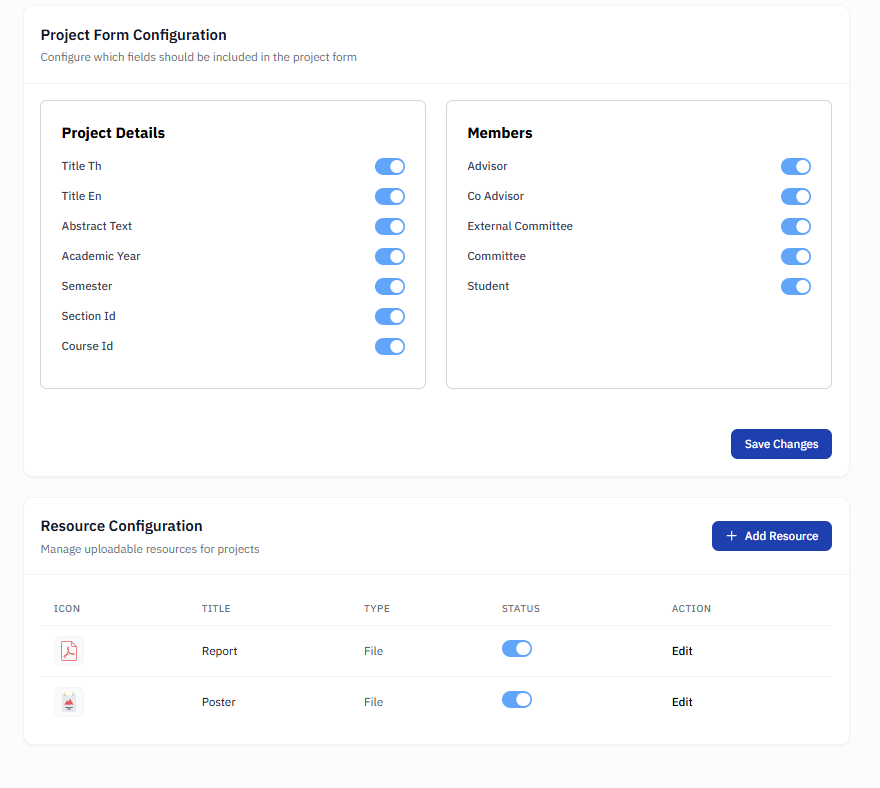
\includegraphics[width=100mm, keepaspectratio ]{pictures/project_box/project_submission_1.png}
        \caption{รูปแบบการส่งโครงงาน}
    \end{figure}

    \begin{figure}[H]
        \centering
        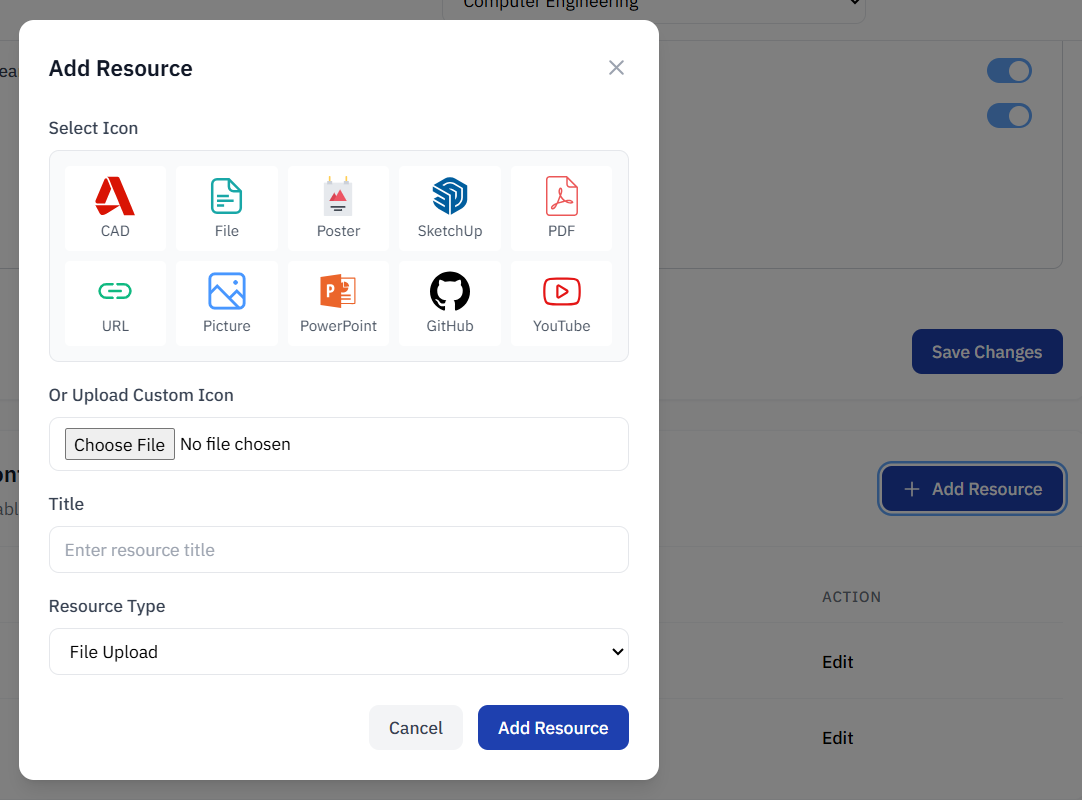
\includegraphics[width=100mm, keepaspectratio ]{pictures/project_box/project_submission_2.png}
        \caption{กำหนดสิ่งที่นักศึกษาต้องส่งในโครงงานของแต่ละสาขา เช่น รายงาน, โค้ด, ฯลฯ}
    \end{figure}
    \newpage
    \item \textbf{จัดการคณาอาจารย์ในสาขา (Manage Staff): } เจ้าหน้าที่สามารถจัดการข้อมูลของอาจารย์ในสาขาได้
    \begin{figure}[H]
        \centering
        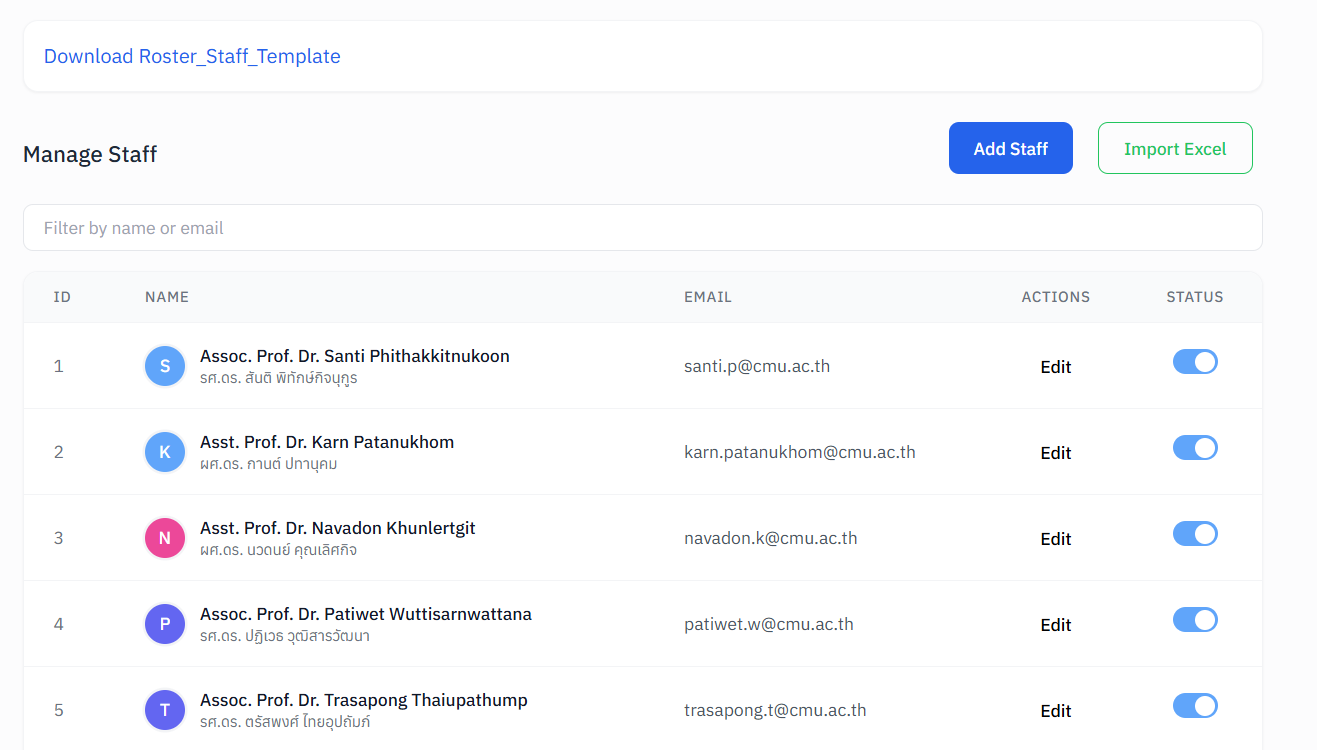
\includegraphics[width=100mm, keepaspectratio ]{pictures/project_box/staff_list.png}
    \end{figure}
    \begin{figure}[H]
        \centering
        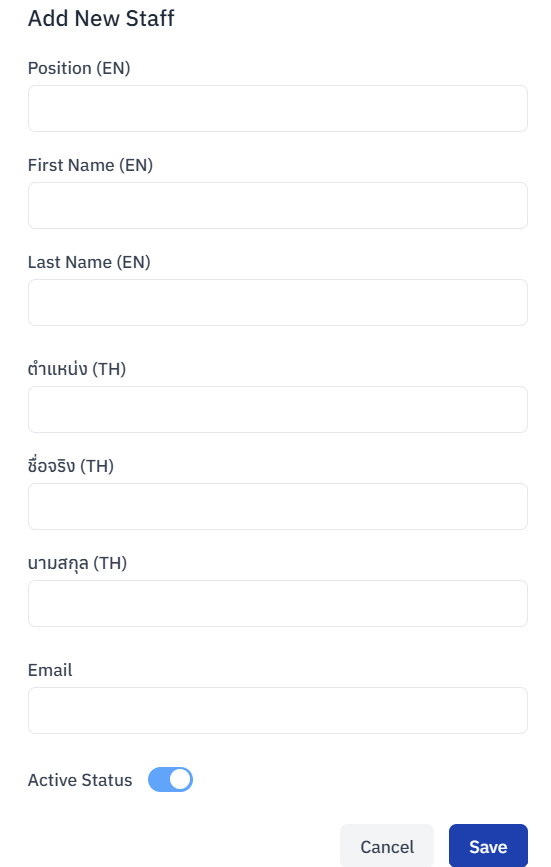
\includegraphics[width=100mm, keepaspectratio ]{pictures/project_box/add_staff.png}
    \end{figure}
    \begin{figure}[H]
        \centering
        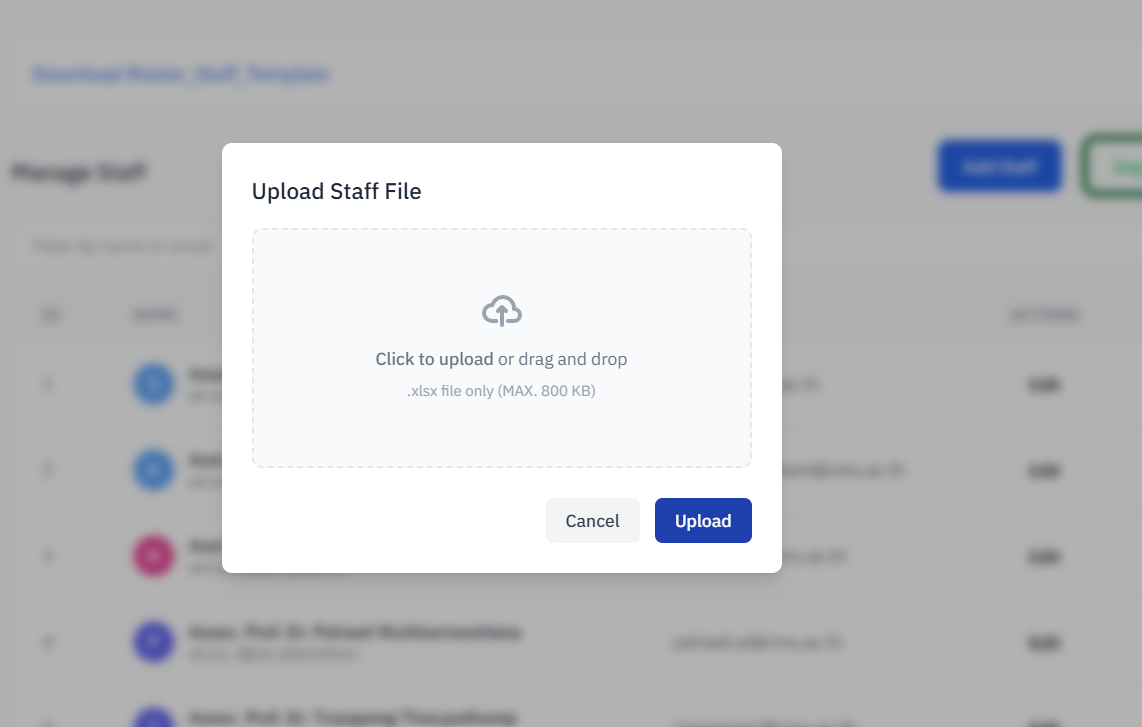
\includegraphics[width=100mm, keepaspectratio ]{pictures/project_box/add_staff_excel.png}
        \caption{ตัวอย่างไฟล์ Excel สำหรับนำเข้าข้อมูลอาจารย์}
    \end{figure}
    \begin{figure}
        \centering
        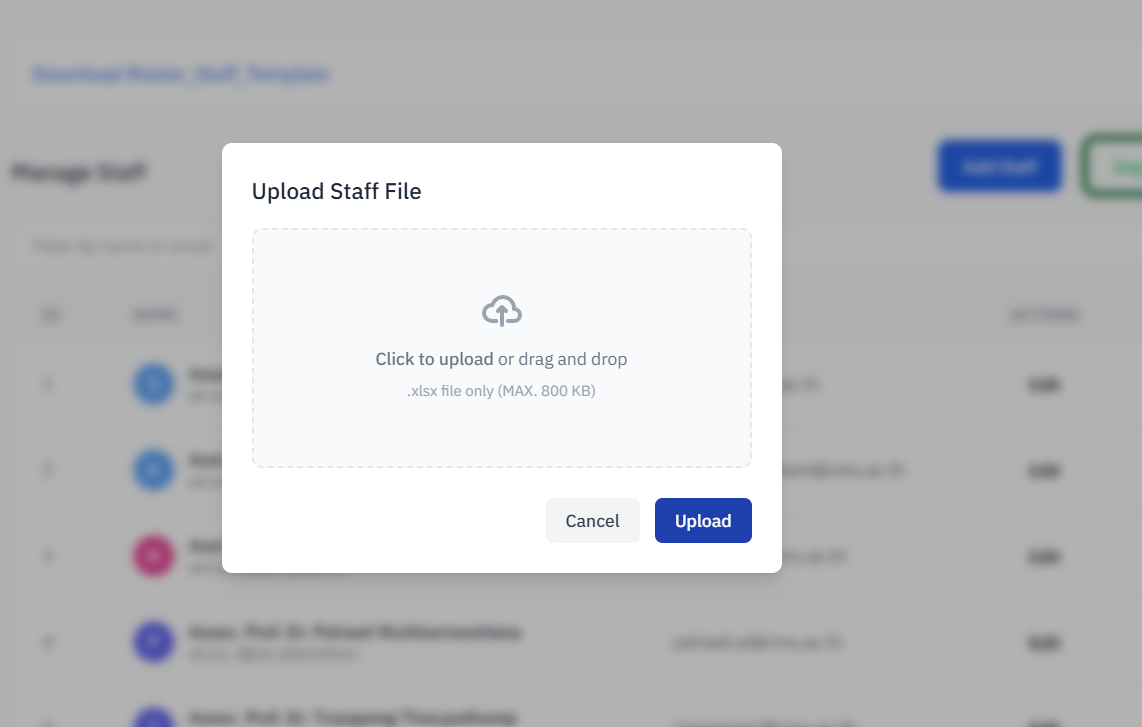
\includegraphics[width=100mm, keepaspectratio ]{pictures/project_box/add_staff_excel.png}
        \caption{เพิ่มข้อมูลอาจารย์ โดยการนำเข้าข้อมูลจากไฟล์ Excel ที่ได้จากสำนักทะเบียน} 
    \end{figure}
    \begin{figure}[H]
        \centering
        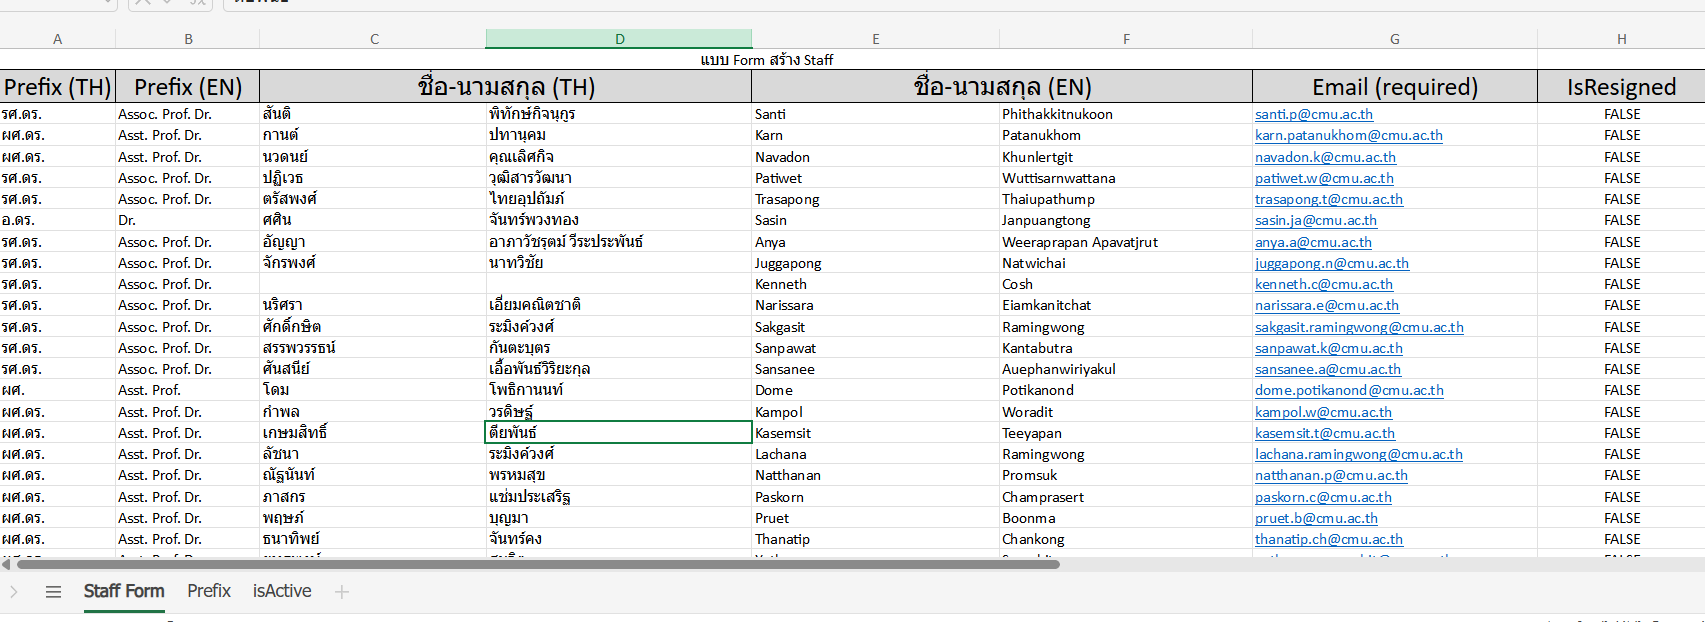
\includegraphics[width=140mm, keepaspectratio ]{pictures/project_box/staff_excel_template.png}
        \caption{ตัวอย่างไฟล์ Excel สำหรับนำเข้าข้อมูลอาจารย์} 
    \end{figure}   
\end{enumerate}
\newpage
\item \textbf{\Large ผู้ดูแลระบบแพลตฟอร์ม (Super Admin): } สามารถจัดการข้อมูลของสาขาและโครงงานทั้งหมดในระบบ รวมถึงจัดการสิทธิ์ให้กับเจ้าหน้าที่ประจำสาขา
\begin{figure}[H]
    \centering
    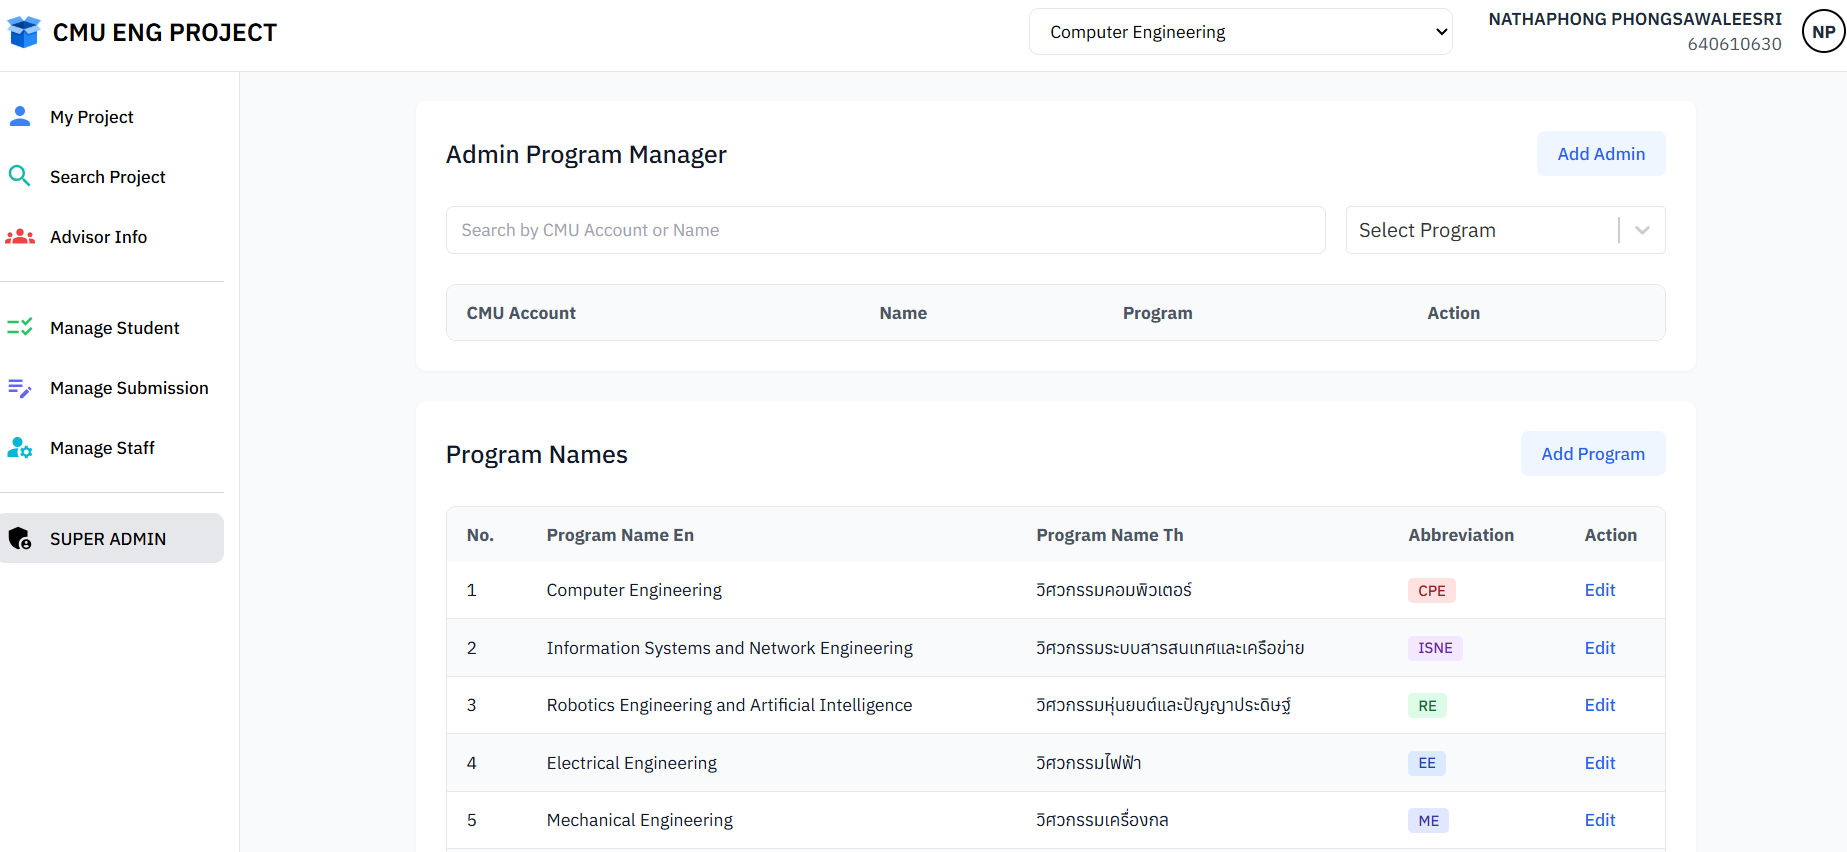
\includegraphics[width=130mm, keepaspectratio ]{pictures/project_box/super_admin.png}
\end{figure}
\begin{figure}[H]
    \centering
    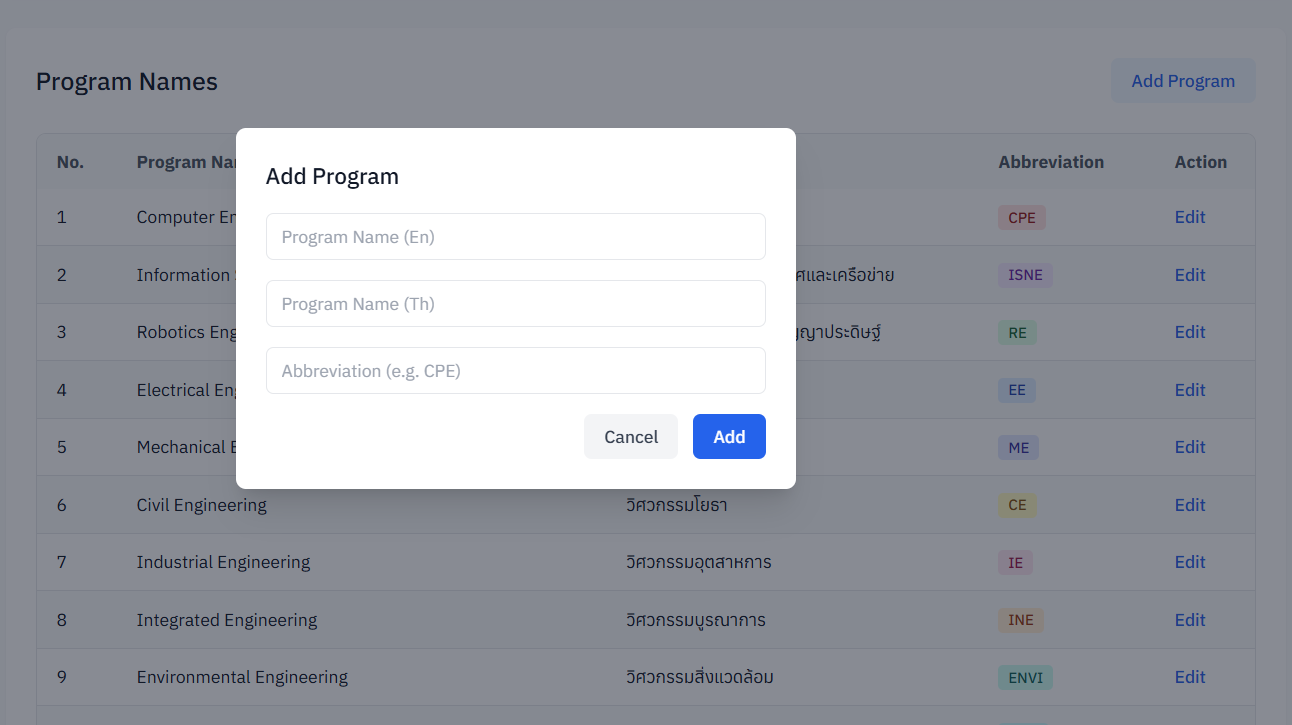
\includegraphics[width=130mm, keepaspectratio ]{pictures/project_box/manage_program.png}
    \caption{จัดการข้อมูลสาขา}
\end{figure}
\begin{figure}[H]
    \centering
    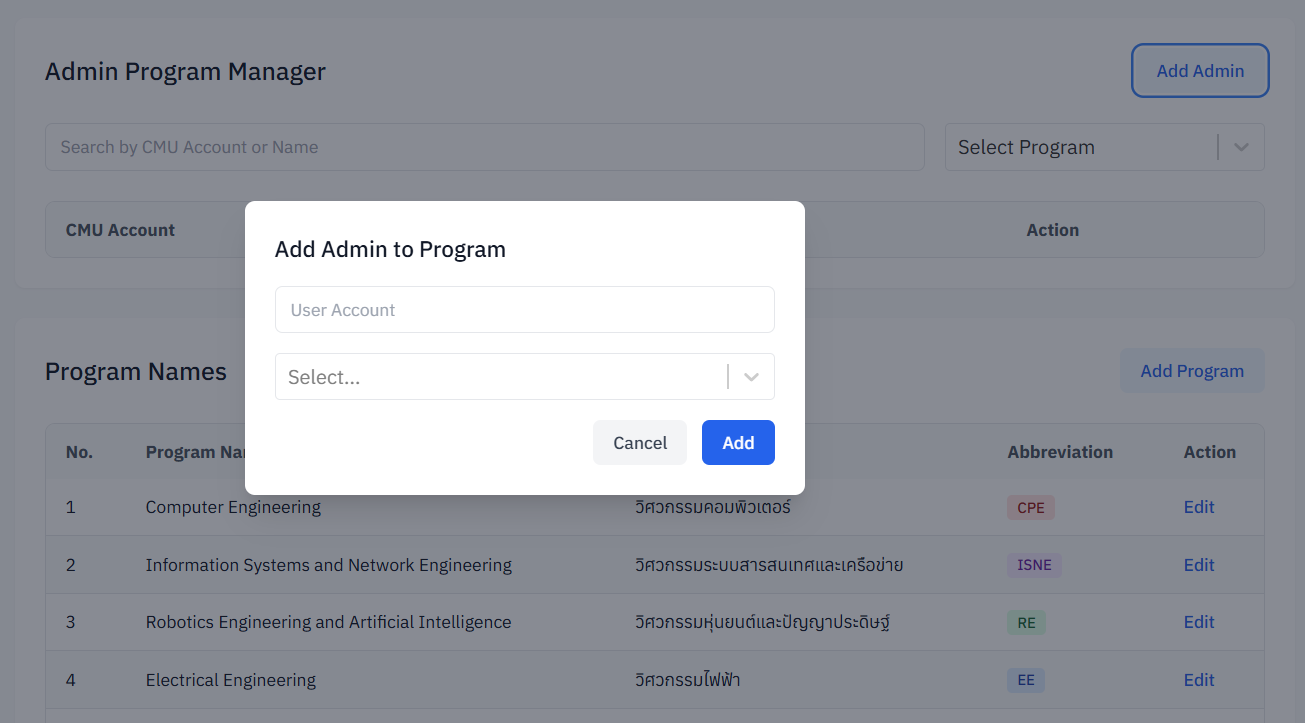
\includegraphics[width=130mm, keepaspectratio ]{pictures/project_box/add_program_admin.png}
    \caption{เพิ่มเจ้าหน้าที่ประจำสาขา}
\end{figure}
\end{itemize}
% \section{appendix}
